%
% $RCSfile: abstraction.tex,v $
%
% Copyright (C) 2002-2008. Christian Heller.
%
% Permission is granted to copy, distribute and/or modify this document
% under the terms of the GNU Free Documentation License, Version 1.1 or
% any later version published by the Free Software Foundation; with no
% Invariant Sections, with no Front-Cover Texts and with no Back-Cover
% Texts. A copy of the license is included in the section entitled
% "GNU Free Documentation License".
%
% http://www.cybop.net
% - Cybernetics Oriented Programming -
%
% http://www.resmedicinae.org
% - Information in Medicine -
%
% Version: $Revision: 1.1 $ $Date: 2008-08-19 20:41:05 $ $Author: christian $
% Authors: Christian Heller <christian.heller@tuxtax.de>
%

\subsection{Abstraction}
\label{abstraction_heading}
\index{Abstractions of Human Thinking}
\index{Item}
\index{Category}
\index{Compound}

Humans understand their environment by building simplified models (concepts) of
it. These are based on fundamental \emph{Abstractions} like \emph{Item},
\emph{Category} or \emph{Compound} (figure \ref{abstraction_figure}), which are
the topic of this section. Part of it was already published in \cite{heller2004}.

\begin{figure}[ht]
    \begin{center}
        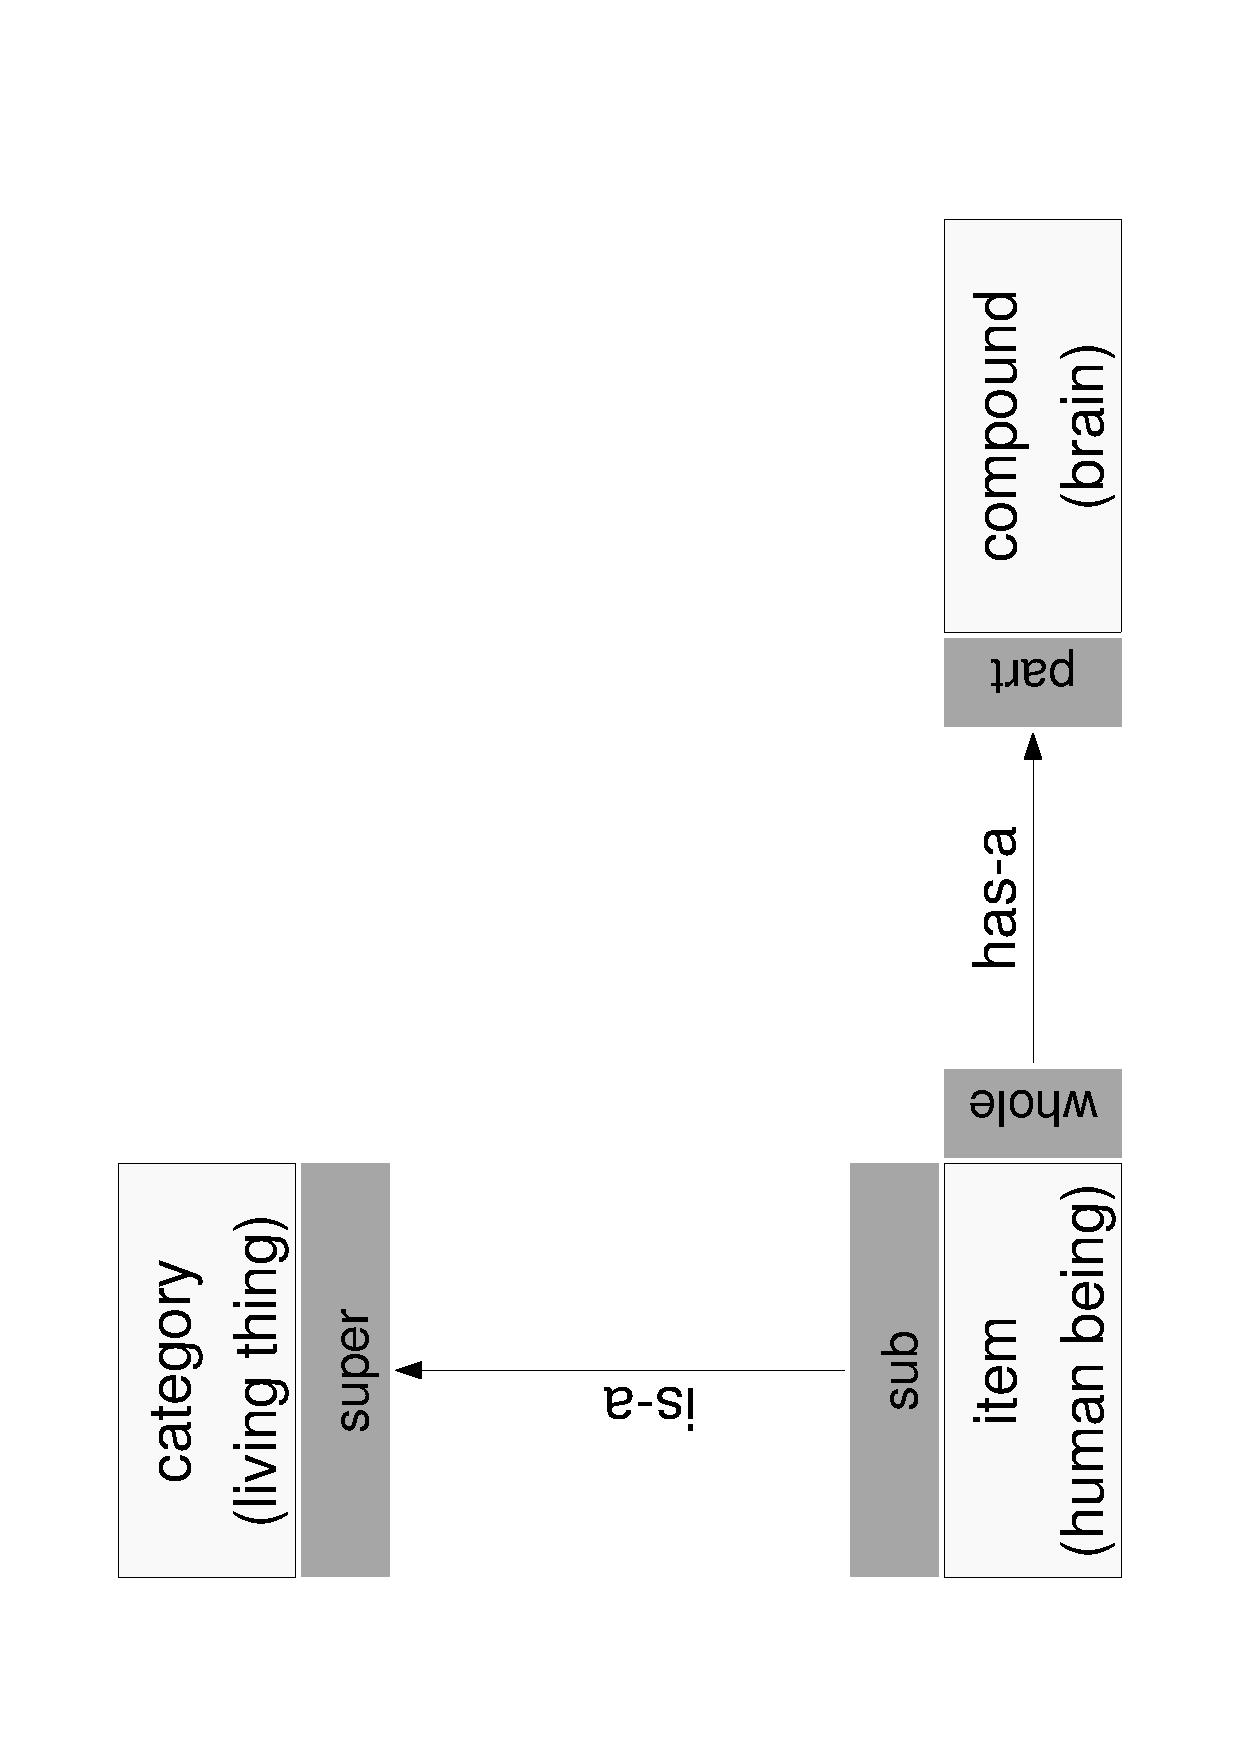
\includegraphics[scale=0.3,angle=-90]{graphic/abstraction.pdf}
        \caption{Abstractions of Human Thinking}
        \label{abstraction_figure}
    \end{center}
\end{figure}

%
% $RCSfile: item.tex,v $
%
% Copyright (c) 2001-2004. Christian Heller. All rights reserved.
%
% No copying, altering, distribution or any other actions concerning this
% document, except after explicit permission by the author!
% At some later point in time, this document is planned to be put under
% the GNU FDL license. For now, _everything_ is _restricted_ by the author.
%
% http://www.cybop.net
% - Cybernetics Oriented Programming -
%
% http://www.resmedicinae.org
% - Information in Medicine -
%
% @author Christian Heller <christian.heller@tuxtax.de>
%

\subsection{Item}
\label{item_heading}

As first and most important abstraction, the human brain divides its real-world
environment into discrete \emph{Items}. Physicists call smaller items \emph{Particle}.
Plenty of other synonyms exist. Software developers often talk of \emph{Object}.
This document preferrably uses the more neutral name \emph{Item}, since models
are created not only of objects but also of \emph{Subjects}.

Behavioural psychologists talk of this ability as \emph{Discrimination}. It commonly
focuses on a specific real world phenomenon, leaving out parameters which are not
interesting in the given context. This is necessary because otherwise, a brain
would have to model and capture the whole universe (with every single particle
being duplicated), which is obviously impossible. As example, a \emph{Human Being}
as item is stated (in parentheses) in figure \ref{human_thinking_figure}.

Not only human beings, but also some higher animal species (like apes) are able
to \emph{discriminate} their environment and to form terms to name it.
Additionally, they have a primitive \emph{Self Concept}, that is a term for
their own personality. However, their cognitive abilities are limited in that
concepts are only available in the presence of the corresponding item. Jaeger
\cite{jaeger} calls that \emph{Online Thinking}; cognition scientists speak of
\emph{Terms of first Order} or \emph{Sensoric Type of Terms}.

Contrary to this, the more advanced \emph{Offline Thinking} allows humans to
think about items they currently cannot sense. Cognition scientists here speak of
\emph{Terms of second Order}. They became possible by \emph{associating} sensoric
signals with terms of a language. The resulting \emph{Net of Associations} brought
a number of advantages \cite{jaeger}:

\begin{itemize}
    \item{\emph{Decoupling} thinking from immediate motoric reaction}
    \item{\emph{Time Index} in scenes so that past memories can be\\
        recalled, the future be planned}
    \item{\emph{Dual Representation} of online and offline contents}
    \item{\emph{Self Awareness} thanks to online and offline thinking}
    \item{\emph{Associations} increasing the expressiveness of terms}
\end{itemize}

%
% $RCSfile: category.tex,v $
%
% Copyright (C) 2002-2008. Christian Heller.
%
% Permission is granted to copy, distribute and/or modify this document
% under the terms of the GNU Free Documentation License, Version 1.1 or
% any later version published by the Free Software Foundation; with no
% Invariant Sections, with no Front-Cover Texts and with no Back-Cover
% Texts. A copy of the license is included in the section entitled
% "GNU Free Documentation License".
%
% http://www.cybop.net
% - Cybernetics Oriented Programming -
%
% http://www.resmedicinae.org
% - Information in Medicine -
%
% Version: $Revision: 1.1 $ $Date: 2008-08-19 20:41:05 $ $Author: christian $
% Authors: Christian Heller <christian.heller@tuxtax.de>
%

\subsubsection{Category}
\label{category_heading}
\index{Category}
\index{Offline Thinking}
\index{Terms of Second Order}
\index{Categorisation}
\index{Type}
\index{Class}
\index{Common Characteristics}
\index{Systematics of Nature}
\index{Classification}
\index{Systematics}
\index{Generalisation}
\index{Specialisation}
\index{Is-a Relationship}
\index{Super Category}
\index{Sub Category}
\index{Parent Category}
\index{Child Category}
\index{Object Oriented Programming}
\index{OOP}
\index{Inheritance}

Offline thinking (in terms of second order) enables humans not only to
discriminate items but also to \emph{categorise} them into superior groups.
Since it is impossible to exactly model the real world in complete, compromises
have to be made: People do not model every single item in their minds but rather
group them into \emph{Types} (\emph{Classes}) of common characteristics.

\begin{figure}[ht]
    \begin{center}
        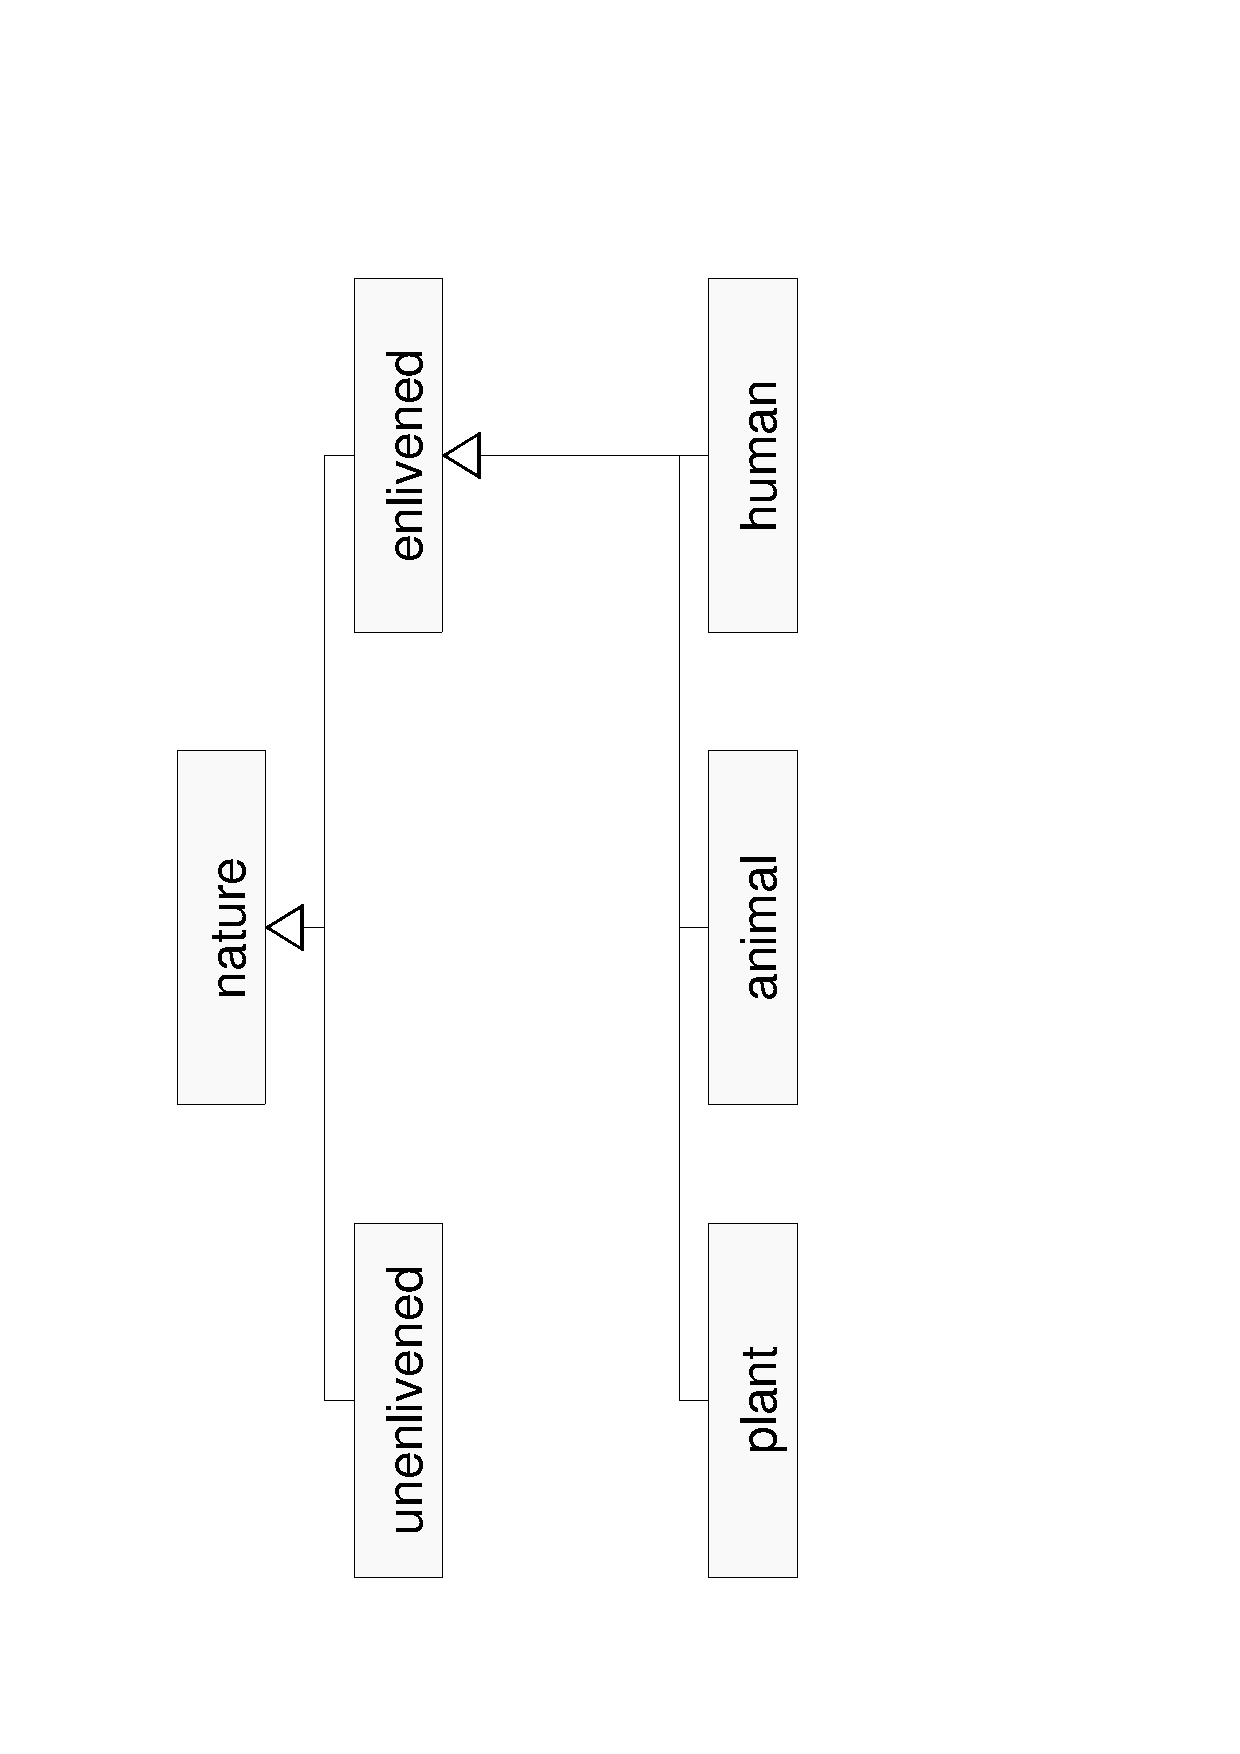
\includegraphics[scale=0.3,angle=-90]{graphic/nature.pdf}
        \caption{Systematics of Nature}
        \label{nature_figure}
    \end{center}
\end{figure}

This kind of classification stems from the earliest days of ancient science.
\emph{Plato}'s (429-347 B.C.) pupil \emph{Aristotle} (384-322 B.C.), being the
teacher of \emph{Alexander the Great}, was the first philosopher who logically
captured and organised the world. It was him who sorted items into clear groups
which he called \emph{Categories}. And it was him who first distinguished
between \emph{enlivened} and \emph{unenlivened} nature; who parted living forms
into \emph{Plants}, \emph{Animals} and \emph{Humans}. The science of biology
calls this classification a \emph{Systematics} (figure \ref{nature_figure}).

\emph{Categorisation} (classification) can be seen from two sides, depending on
what direction of that relationship one wants to emphasise. Taking Aristotle's
examples, \emph{Living Thing} would be a \emph{Generalisation} of \emph{Plants},
\emph{Animals} and \emph{Humans}. \emph{Animal} would be a \emph{Specialisation}
of \emph{Living Thing}.

Software developers often call categorisation an \emph{is-a} relationship and
talk of \emph{Super} and \emph{Sub} categories (sometimes also \emph{Parent}
and \emph{Child} categories). Section \ref{inheritance_heading} described how
\emph{Object Oriented Programming} (OOP) uses categorisation to let a sub class
inherit attributes and methods from its super class.

%
% $RCSfile: compound.tex,v $
%
% Copyright (c) 2001-2004. Christian Heller. All rights reserved.
%
% No copying, altering, distribution or any other actions concerning this
% document, except after explicit permission by the author!
% At some later point in time, this document is planned to be put under
% the GNU FDL license. For now, _everything_ is _restricted_ by the author.
%
% http://www.cybop.net
% - Cybernetics Oriented Programming -
%
% http://www.resmedicinae.org
% - Information in Medicine -
%
% @author Christian Heller <christian.heller@tuxtax.de>
%

\subsection{Compound}
\label{compound_heading}

\emph{Composition} is the third kind of abstraction that humans use to understand
their environment. It is an important instrument for the human mind to associate
information, that is to acquire, store and recall \emph{Knowledge}. Every item is
recognized as a \emph{Compound} of smaller items and can therefore also be called
\emph{Tree} or \emph{Hierarchy}. The subject of \emph{Artificial Intelligence} (AI)/
\emph{Knowledge Engineering} talks of \emph{Concept} or \emph{Schema}.

In software design, the terms \emph{Parent} and \emph{Child} are often used to
describe both, the items in a composition as well as the items in a categorization
relationship (section \ref{category_heading}).
To avoid misunderstandings, this document sticks to the terms \emph{Super} and
\emph{Sub} for categorization and to the terms \emph{Whole} and \emph{Part}
\cite{sowa} for composition. Yet other terms to describe items of a composition
would be \emph{Container} and \emph{Element}.

To stick with the example of a \emph{Human Being}, one could say that it is
composed of \emph{Organs} such as \emph{Eye}, \emph{Ear}, \emph{Heart},
\emph{Brain}, \emph{Arm} and further, also smaller parts. Other examples are the
concept of an \emph{Atom} consisting of a \emph{Core} and \emph{Electrons} or
that of a physical \emph{Book} composed of a \emph{Paperback Cover} and
\emph{Paper Pages}.
However, knowledge representation always depends on what one wants to express in
which context. The \emph{Book}, for example, can be represented in many other
ways. Logically, it is usually separated into \emph{Part}, \emph{Chapter},
\emph{Section}, \emph{Paragraph}, \emph{Sentence}, \emph{Word} and \emph{Character}.

It is important to note the \emph{unidirectional} kind of relations: A human
being is composed of organs but an organ is never composed of a human being!

Not only \emph{static} items represent a compound; \emph{dynamic} items are
hierarchical as well. The process \emph{Take Book from Library}, for example,
may have the following structure:

\begin{itemize}
    \item{Check Catalogue}
    \begin{itemize}
        \item{Investigate suitable Books}
        \item{Note Registration Number}
    \end{itemize}
    \item{Organize Book}
    \begin{itemize}
        \item{Look for Shelf}
        \item{Take off Book}
    \end{itemize}
    \item{Borrow Book}
\end{itemize}

Returning to human thinking, one realizes that in the end, everything in universe
can be put into variable hierarchical models, that is consists of smaller items
and belongs to a bigger item. From the physical point of view, nobody knows where
this hierarchy really stops, towards \emph{Microcosm} as well as towards
\emph{Macrocosm}. There is no \emph{absolute}, \emph{basic} item.
A \emph{Particle} as concept exists only in the human mind, placed somewhere
between micro- and macrocosm, with hypothetic borders.

